%begin_custom_header
\documentclass[11pt]{article}	% RECOMB: "at least 11 point font size on U.S. standard 8 1/2 by 11 inch paper with no less than one inch margin all around."				
\usepackage[utf8]{inputenc}   % umlauts etc.
\usepackage[english]{babel}
\usepackage [autostyle, english = american]{csquotes}
\MakeOuterQuote{"}
\usepackage{hyperref}
\usepackage{array}
% ----------------------------------
\usepackage[backend=biber,style=nature,sorting=none,url=false]{biblatex}
% url = false. There are also isbn, doi etc., similar options. 
\addbibresource{/Users/mohammedalshamrani/Downloads/School/Waldispul/Publishing/z-misc/zotero-library/my_library.bib}
% ----------------------------------
% Citation style 	biblatex stylename
% ----------------------------------
% 	ACS				chem-acs
% 	AIP				phys (*)
% 	Natur			nature
% 	Science			science
% 	IEEE			ieee
% 	Chicago			chicago-authordate
% 	MLA				mla
% 	APA				apa
% ----------------------------------
% sorting options:
% ----------------------------------
%	nty 		Sort by name, title, year.
%	nyt 		Sort by name, year, title.
%	nyvt 		Sort by name, year, volume, title.
%	anyt 		Sort by alphabetic label, name, year, title.
%	anyvt 		Sort by alphabetic label, name, year, volume, title.
%	ynt 		Sort by year, name, title.
%	ydnt 		Sort by year (descending), name, title.
%	none 		Do not sort at all. All entries are processed in citation order.
% ----------------------------------
\newcommand{\harpoon}{\overset{\rightharpoonup}}
\newtheorem{theorem}{Theorem}
\usepackage{verbatim} % multiline comment
\usepackage{graphicx}
\graphicspath{{/Users/mohammedalshamrani/Downloads/School/Waldispul/Publishing/Paper_04/fig/}}
\setlength\fboxsep{0pt} % figure border padding
\setlength\fboxrule{1pt} % figure outline
\usepackage[fleqn]{amsmath}  % also \documentclass[fleqn]{article}
\usepackage[margin=1in]{geometry}
\abovedisplayskip=0pt
\abovedisplayshortskip=0pt
\belowdisplayskip=0pt
\belowdisplayshortskip=0pt
\setlength{\mathindent}{0pt}
\usepackage{amsfonts} % for R (real numbers)
\usepackage{float}
\usepackage[font=scriptsize,labelfont=bf]{caption}

\usepackage[percent]{overpic}
\usepackage[export]{adjustbox}
% ----------------------------------
%Squeezing the Vertical White Space
%http://www.terminally-incoherent.com/blog/2007/09/19/latex-squeezing-the-vertical-white-space/
% 	THIS FIXES THE PROBLEM OF SUBSECTIONS STARTING IN A NEW PAGE
\setlength{\parskip}{0pt}
\setlength{\parsep}{10pt}
\setlength{\headsep}{0pt}
\setlength{\topskip}{0pt}
\setlength{\topmargin}{0pt}
\setlength{\topsep}{0pt}
\setlength{\partopsep}{10pt}
\usepackage[compact]{titlesec}
\titlespacing{\section}{0pt}{*2}{*2} % {left margin} {above-skip} {below-kip} , The * notation replaces the formal notation using plus/minus and etc. 
\titlespacing{\subsection}{0pt}{*1}{*1}
\titlespacing{\subsubsection}{0pt}{*1}{*1}
% ----------------------------------
\newenvironment{absolutelynopagebreak}
  {\par\nobreak\vfil\penalty0\vfilneg
   \vtop\bgroup}
  {\par\xdef\tpd{\the\prevdepth}\egroup
   \prevdepth=\tpd}
% ----------------------------------
\newcommand{\bfl}{\begin{flushleft}}
\newcommand{\efl}{\end{flushleft}}
\newcommand{\mys }{\hspace{0.1cm}}
\newcommand{\figfont}{\footnotesize}

\usepackage{geometry} %
%begin_custom_header
\usepackage[table]{xcolor} % for \arrayrulecolor{yellow}, changes hline and vline colors
\usepackage{array}
\usepackage{lmodern}
\usepackage{multirow, booktabs} % http://tex.stackexchange.com/questions/328793/table-custom-cell-vertical-alignment					
%end_custom_header
\begin{document}
%begin_custom_content
\section{Results} \label{sec:results}
			Here we present ultraviolet images of gel electrophoresis showing DNA templates, RNA transcript, and RNA ligation results. 
			Figure \ref{fig:results}  (a) and (b) show double-stranded DNA (dsDNA) templates encoding nodes N0 to N6 and 
			edges E0 $\rightarrow$E1 to E5 $\rightarrow$E6, respectively.  The inset shows the reference molecular marker (ladder) 
			used to verify that the observed length of each dsDNA template appears on the gel at the expected length. The PCR product of 
			N6 dsDNA template (Figure 4a, well 7 from the left) shows erroneous bands, so the correct band is gel-excised under ultraviolet 
			visualization and purified using the crush-and-soak method [28]. The transcription of N6 results in a clean band corresponding 
			to the expected length of 98-nt (well 8 in Figure 4b). RNA transcripts of E0$\rightarrow$E1, E1$\rightarrow$E2, E2$\rightarrow$E3, 
			E3$\rightarrow$E4, E4$\rightarrow$E5, and E5$\rightarrow$E6 in Figure 4b (wells 10-15) show smears as they are loaded immediately 
			from in-vitro transcription reaction without purification, while purified transcripts of N0 to N6  are purified prior to loading 
			(Zymo Research kit \# R1019). The length of an RNA transcript is the length of its corresponding DNA template minus the T7 
			promoter region (25-bp) and leading sequence (25-32 bp). For example, the length of N6’s RNA transcript 
			is 98-nt = 152 - 29 – 25 (152-bp total dsDNA template length – 29-bp (leading) –  25-bp T7 (promoter)).
			\begin{figure}[H]
				\begin{table}[H]
				    \arrayrulecolor[HTML]{ffffff}% midrule is used to create vertical space between rows, make it white. blue = 0a84f7
					\centering
					% multirow is used to control vertical alignment within a cell: http://tex.stackexchange.com/questions/328793/table-custom-cell-vertical-alignment
					\begin{tabular}{{  | @{}p{.6\textwidth} | p{.1\textwidth}@{} |   }}				
						\toprule
						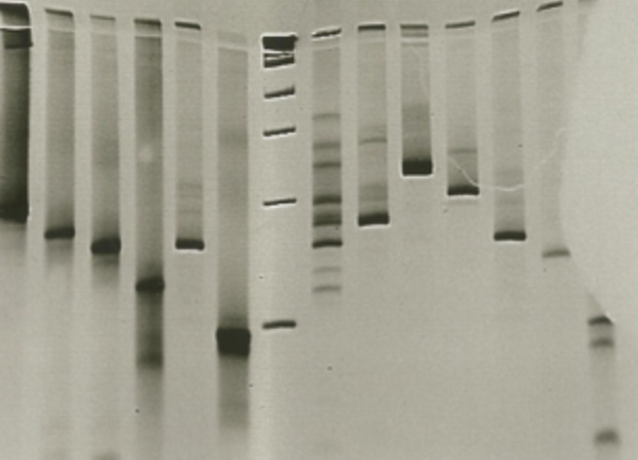
\includegraphics[scale=.75, center]{02_results/dsDNA.pdf}  
						& 
						\multirow{-10}{\linewidth}{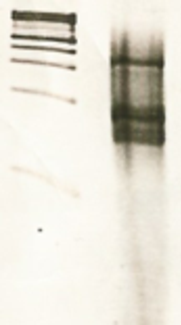
\includegraphics[scale=.6, center]{02_results/RNA_ligation.pdf} } 
						\\
						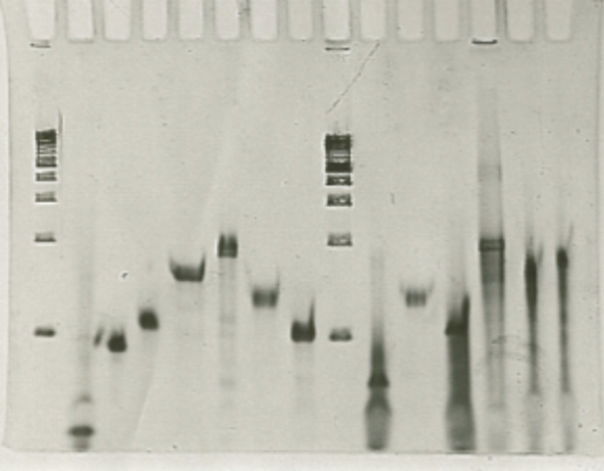
\includegraphics[scale=.75, center]{02_results/RNA.pdf}   
						& 
						\multirow{-10}{\linewidth}{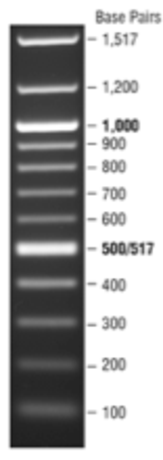
\includegraphics[scale=.5, center]{02_results/ladder.pdf}  }  
						%\\ \midrule\midrule\midrule\midrule  % midrule is thicker than \hline
						\\ \bottomrule
					\end{tabular}	
				\end{table}		
				\caption{Gel electrophoresis results of DNA templates, RNA transcripts, and RNA ligation products. 
							Inset: standard 100-bp molecular marker (NEB). (a) Double-stranded DNA (dsDNA) template strands encoding 
							for nodes \& edges, run on 4\% non-denaturing polyacrylamide gel. Wells left to right, w1-w7: templates 
							N0 to N6 of lengths 91, 134, 151, 194, 224, 170, and 152 base pairs (bp), respectively; w8: marker (inset); 
							w9-14: partial set of dsDNA templates encoding for edges E0$\rightarrow$E1, E1$\rightarrow$E2, E2$\rightarrow$E3, 
							E3$\rightarrow$E4, E4$\rightarrow$E5, and E5$\rightarrow$E6 of lengths 70, 123, 98, 182, 133, 149 bp, respectively.  
							N6 template (well 7) shows erroneous PCR byproducts subsequently excluded by excising the correct 
							band \& crush-and-soak purifying it [28]. Each sequence is primed upstream with a T7 promoter. 
							(b) Partial set of purified in-vitro transcribed RNA nodes \& edges run on 4\% TBE-Urea denaturing 
							polyacrylamide gel; left to right, w1/w9: marker (inset), w2-w8: RNA transcripts of N0 to N6 with 
							lengths 44, 87, 102, 147, 177, 120, 98-nt, respectively; w10-w15: RNA transcripts of edges E0$\rightarrow$E1, 
							E1$\rightarrow$E2, E2$\rightarrow$E3, E3$\rightarrow$E4, E4$\rightarrow$E5, and E5$\rightarrow$E6 
							with lengths 70, 123, 98, 182, 133, 149-nt, respectively. (c) Example RNA ligation; w1: marker (inset); 
							w2: ligation of N3 RNA transcript (147-nt) to N4 (177-nt) by splint ligation with edge 3$\rightarrow$E4 
							transcript (182-nt) to form a 324-nt RNA strand (ligation product). 
							}
				\label{fig:results}
			\end{figure}
%end_custom_content
\printbibliography
\end{document}